%!TeX root=../tese.tex
%("dica" para o editor de texto: este arquivo é parte de um documento maior)
% para saber mais: https://tex.stackexchange.com/q/78101

\chapter{Algoritmo totalmente dinâmico para MSF}
\label{chapter:fully-MSF}

Neste capítulo, estudaremos o algoritmo totalmente dinâmico para MSF, o qual chamaremos de \textbf{MSF dinâmica}. Como este algoritmo não será implementado em nosso estudo, apresentaremos apenas a ideia por trás dele, de como podemos manter o peso mínimo de uma MSF de um grafo $G$ que suporte adição e remoção de arestas. Inicialmente, será descrito o funcionamento das \textbf{top trees}, estruturas de dados que serão usadas na construção da MSF dinâmica. Estas estruturas estão descritas na Seção~2.2 do artigo de Holm, de Lichtenberg e Thorup~\cite{jacob_holm}.

\section{Top trees}

A construção de uma top tree é baseada em um par ($T$, $\partial T$), onde $T$ é uma árvore e $\partial T$ é um conjunto que contém no máximo dois vértices de $T$, que são chamados vértices da fronteira (\textit{external boundary vertices}), como se pode ver na Figura~\ref{fig:top-tree-pair-representation}.

\begin{figure}[H]
    \centering
    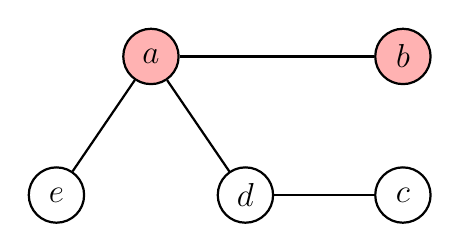
\begin{tikzpicture}
        [scale=0.8, node/.style={circle,draw,minimum size=2em, thick, font=\large},
        edge/.style={thick, black},
        reserve/.style={red, thick},
        removed/.style={black, thick, dashed}, 
        inner sep=0pt]

        \node[node, fill=red!30] (a) at (0,1.5) {$a$};
        \node[node, fill=red!30] (b) at (4,1.5) {$b$};
        \node[node] (c) at (4,-0.7) {$c$};
        \node[node] (d) at (1.5,-0.7) {$d$};
        \node[node] (e) at (-1.5,-0.7) {$e$};

        \draw[edge] (a) -- (b) node[midway, above] {};
        \draw[edge] (c) -- (d) node[midway, above] {};
        \draw[edge] (d) -- (a) node[midway, above] {};
        \draw[edge] (a) -- (e) node[midway, above] {};

    \end{tikzpicture}
    \caption{Representação de uma árvore $T$ de $5$ vértices. Os vértices pintados em vermelho são vértices da fronteira de $T$, ou seja, formam o conjunto $\partial T$.}
    \label{fig:top-tree-pair-representation}
\end{figure}

Assim, dado ($T$, $\partial T$), qualquer subárvore $C$ de $T$ tem um conjunto $\partial_{(T, \partial T)}C$ de vértices da fronteira, que são vértices de $C$ que estão ou em $\partial T$ ou são incidentes a uma aresta de $T$ saindo de $C$, como se pode ver no exemplo da Figura~\ref{fig:top-tree-subtree-option1}.

\begin{figure}[H]
    \centering
    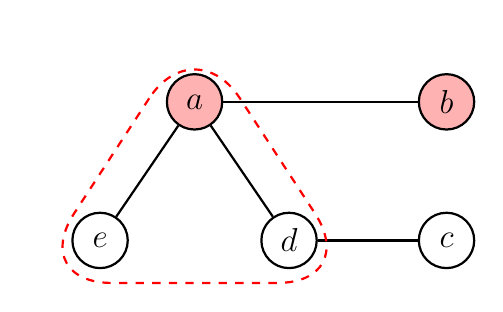
\begin{tikzpicture}
        [scale=0.8, node/.style={circle,draw,minimum size=2em, thick, font=\large},
        edge/.style={thick, black},
        reserve/.style={red, thick},
        removed/.style={black, thick, dashed}, 
        inner sep=0pt]

        \node[node, fill=red!30] (a) at (0,1.5) {$a$};
        \node[node, fill=red!30] (b) at (4,1.5) {$b$};
        \node[node] (c) at (4,-0.7) {$c$};
        \node[node] (d) at (1.5,-0.7) {$d$};
        \node[node] (e) at (-1.5,-0.7) {$e$};

        \draw[edge] (a) -- (b) node[midway, above] {};
        \draw[edge] (c) -- (d) node[midway, above] {};
        \draw[edge] (d) -- (a) node[midway, above] {};
        \draw[edge] (a) -- (e) node[midway, above] {};
        
        % P1: Top Vertex (above node 'a')
        \coordinate (P1) at ([yshift=20pt]a.north); 
        
        % P2: Bottom-Left Vertex (left of 'e' and slightly below it, using calc for precision)
        \coordinate (P2) at ([xshift=-23pt, yshift=-10pt]e.south west);
        
        % P3: Bottom-Right Vertex (right of 'd' and slightly below it, using calc for precision)
        \coordinate (P3) at ([xshift=23pt, yshift=-10pt]d.south east);

        % --- Draw the Dashed Triangular Outline ---
        
        % Connect the invisible coordinates with rounded corners
        \draw[dashed, thick, red, rounded corners=30pt] 
            (P1) -- (P2) -- (P3) -- cycle;

        % \draw[dashed, thick, red] (e) -- (a) -- (d) -- cycle;
    \end{tikzpicture}
    \caption{Representação de uma árvore $T$ de $5$ vértices. Os vértices pintados em vermelho são vértices da fronteira de $T$. A região demarcada em vermelho representa a subárvore $C$ contendo os vértices $a$, $e$ e $d$ e as arestas $ae$ e $ad$. Neste exemplo, note que os vértices da fronteira de $C$ são $a$ e $d$.}
    \label{fig:top-tree-subtree-option1}
\end{figure}

Uma subárvore $C$ é chamado \textbf{cluster} de ($T$, $\partial T$) se ela possuir no máximo dois vértices da fronteira. Assim, por definição, $T$ é um cluster dele mesmo, com $\partial_{(T, \partial T)}T = \partial T$. A subárvore $C$ da Figura~\ref{fig:top-tree-subtree-option1} acima é um cluster, pois ele possui apenas dois vértices da fronteira.

Além disso, se $R$ é uma subárvore de $C$, isto é, $\partial_{(C, \partial_{(T, \partial T)}C)}R = \partial_{(T, \partial T)} R$, então $R$ é um cluster  
 de ($C$, $\partial_{(T, \partial T)} C$) se, e somente se, $R$ é um cluster de $(T, \partial T)$. Podemos ver essa situação no exemplo da Figura~\ref{fig:top-tree-cluster-of-cluster}. Para simplificar, denotaremos $\partial_{(T, \partial T)}$ como $\partial$ a partir de agora.

 \begin{figure}[H]
    \centering
    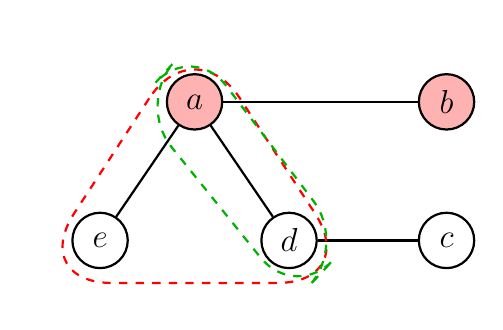
\begin{tikzpicture}
        [scale=0.8, node/.style={circle,draw,minimum size=2em, thick, font=\large},
        edge/.style={thick, black},
        reserve/.style={red, thick},
        removed/.style={black, thick, dashed}, 
        inner sep=0pt]

        \node[node, fill=red!30] (a) at (0,1.5) {$a$};
        \node[node, fill=red!30] (b) at (4,1.5) {$b$};
        \node[node] (c) at (4,-0.7) {$c$};
        \node[node] (d) at (1.5,-0.7) {$d$};
        \node[node] (e) at (-1.5,-0.7) {$e$};

        \draw[edge] (a) -- (b) node[midway, above] {};
        \draw[edge] (c) -- (d) node[midway, above] {};
        \draw[edge] (d) -- (a) node[midway, above] {};
        \draw[edge] (a) -- (e) node[midway, above] {};
        
        % P1: Top Vertex (above node 'a')
        \coordinate (P1) at ([yshift=20pt]a.north); 
        
        % P2: Bottom-Left Vertex (left of 'e' and slightly below it, using calc for precision)
        \coordinate (P2) at ([xshift=-23pt, yshift=-10pt]e.south west);
        
        % P3: Bottom-Right Vertex (right of 'd' and slightly below it, using calc for precision)
        \coordinate (P3) at ([xshift=23pt, yshift=-10pt]d.south east);


        \draw[dashed, thick, red, rounded corners=30pt] 
            (P1) -- (P2) -- (P3) -- cycle;
        % G1: Top-Left point (relative to 'a')
  
        % Top-Left corner (above and to the left of 'a')
        \coordinate (DR1) at ([xshift=-10pt, yshift=18pt]a.north east); 
        
        % Bottom-Left corner (below and to the left of 'a', near 'e')
        \coordinate (DR2) at ([xshift=-17pt, yshift=-10pt]a.north west); 
        
        % Bottom-Right corner (below and to the right of 'd', near 'c')
        \coordinate (DR3) at ([xshift=12pt, yshift=-18pt]d.south west); 
        
        % Top-Right corner (above and to the right of 'd')
        \coordinate (DR4) at ([xshift=17pt, yshift=7pt]d.south east); 

        % --- Draw the Dashed Green Diagonal Rectangle ---
        \draw[dashed, thick, green!70!black, rounded corners=20pt] 
            (DR1) -- (DR2) -- (DR3) -- (DR4) -- cycle;

        % \draw[dashed, thick, red] (e) -- (a) -- (d) -- cycle;
    \end{tikzpicture}
    \caption{Representação de uma árvore $T$ de $5$ vértices. Os vértices pintados em vermelho são vértices da fronteira de $T$. A região demarcada em vermelho representa a subárvore $C$ de $T$, e é cluster de $T$, contendo os vértices $a$, $e$ e $d$ e as arestas $ae$ e $ad$. Já a região demarcada em verde representa a subárvore $R$ de $C$ contendo os vértices $a$ e $d$ e a aresta $ad$, e é cluster de $C$ e de $T$.}
    \label{fig:top-tree-cluster-of-cluster}
\end{figure}

Dizemos que clusters $A$ e $B$ são vizinhos se eles compartilham um único vértice entre eles e se $A \cup B$ é um cluster, como podemos ver na Figura~\ref{fig:clusters-formation-cases}. Assim, definimos uma top tree $\mathcal{T}$ do par ($T$, $\partial T$) como sendo uma árvore binária que respeita o seguinte:

\begin{itemize}
    \item Os vértices de $\mathcal{T}$ são clusters de ($T$, $\partial T$);
    \item As folhas de $\mathcal{T}$ são as arestas de $T$;
    \item Se $C$ é pai de $A$ e de $B$ em $\mathcal{T}$, então $C = A \cup B$ e $A$ e $B$ são vizinhos;
    \item a raiz de $\mathcal{T}$ é a própria árvore $T$.
\end{itemize}

Para um cluster $C$, os vértices em $C\backslash \partial C$ são chamados de vértices internos (\textit{internal vertices}). Se $a$ e $b$ são vértices da fronteira de $C$, o caminho $a \cdots b$ se chama \textit{cluster path} e denotamos por $\pi(C)$. Se $a \neq b$, o cluster é chamado de \textit{path cluster}. 

Dizemos que o cluster $C$ é \textit{path ancestor} do cluster $D$ e $D$ é chamado de \textit{path descendant} de $C$ se ambos forem \textit{path clusters} e $\pi(D) \subseteq \pi(C)$. Note que cada aresta $e \in \pi(C)$ é um \textit{path descendant} de $C$. Um filho que é caminho descendente é um \textit{path child}. Na Figura~\ref{fig:clusters-formation-cases}, apresentamos os quatro casos quando fazemos a união de dois clusters. Em (1), temos dois \textit{path children}. Em (2), temos um \textit{path child}, e zero \textit{path children} em (3) e (4).


\begin{figure}[H]
    \centering
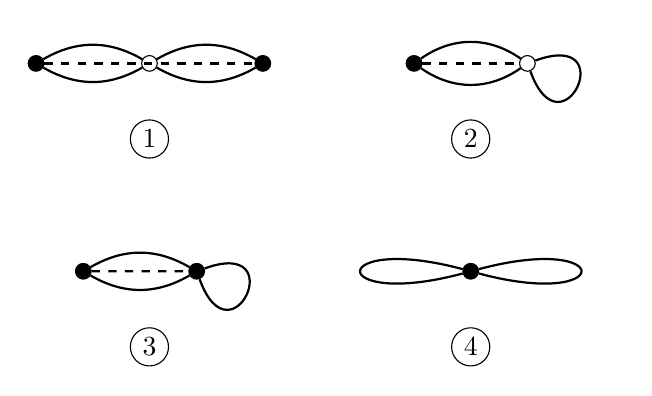
\begin{tikzpicture}[scale=1.2,
    every node/.style={circle, draw, inner sep=2pt},
    boundary/.style={fill=black},
    internal/.style={fill=white},
    edge/.style={thick},
    dashededge/.style={thick, dashed}
]

% (1)
\node[boundary] (a1) at (0,0) {};
\node[internal] (b1) at (1.2,0) {};
\node[boundary] (c1) at (2.4,0) {};

\draw[edge, bend left=30] (a1) to (b1);
\draw[edge, bend right=30] (a1) to (b1);
\draw[edge, bend left=30] (b1) to (c1);
\draw[edge, bend right=30] (b1) to (c1);
\draw[dashededge] (a1) -- (c1);
\node at (1.2, -0.8) {1};

% (2)
\node[boundary] (a2) at (4,0) {};
\node[internal] (b2) at (5.2,0) {};

\draw[edge, bend left=35] (a2) to (b2);
\draw[edge, bend right=35] (a2) to (b2);
\draw[edge, in=290, out=20, looseness=20] (b2) to (b2);
\draw[dashededge] (a2) -- (b2);
\node at (4.6, -0.8) {2};

% (3)
\node[boundary] (a3) at (0.5,-2.2) {};
\node[boundary] (b3) at (1.7,-2.2) {};

\draw[edge, bend left=30] (a3) to (b3);
\draw[edge, bend right=30] (a3) to (b3);
\draw[edge, in=290, out=20, looseness=20] (b3) to (b3);
\draw[dashededge] (a3) -- (b3);
\node at (1.2, -3) {3};

% (4)
\node[boundary] (a4) at (4.6, -2.2) {};

\draw[edge] (a4) edge[loop left, min distance=15mm, looseness=4] (a4);
\draw[edge] (a4) edge[loop right, min distance=15mm, looseness=4] (a4);
\node at (4.6, -3) {4};

\end{tikzpicture}
\caption{Representação da união de dois clusters $A$ e $B$ formando um cluster $C$, e seus quatro diferentes casos. Os vértices pretos são vértices da fronteira de $C$ após a união de $A$ e $B$. Já os vértices brancos são vértices da fronteira de $A$ e de $B$, mas que não tornaram vértices da fronteira de $C$ após a união. A linha tracejada é o caminho do cluster (\textit{cluster path}) formada entre os vértices da fronteira de $C$.}
    \label{fig:clusters-formation-cases}
\end{figure}

Ademais, se $a$ é um vértice de fronteira de $C$ e $C$ possui dois filhos $A$ e $B$, então $A$ é considerado o mais próximo de $a$ se $a \notin B$. Caso $\partial C = \partial A = \partial C$, então o cluster mais próximo é escolhido arbitrariamente.